

AJFS is designed to be, above all else, simple both in its guarantees and in its
implementation. As such, several assumptions were made to keep the scope of the
project manageable. These assumptions allow the design methodology that we used
to be possible, and thus warrant discussion outright.

\subsection{Use Cases and Assumptions}

AJFS is aimed at a use case similar to Dropbox: while multiple users could be
editing files on multiple systems simultaneously, it is primarily designed for a
single user across multiple systems. The emphasis is on data availability across
systems, and is not designed with 'collaborative' uses in mind.

From a network perspective, AJFS assumes that, excepting in the case of a
partition, the nodes in the system will be fully connected (meaning all nodes
can communicate with all others). While a partition is a case we handle, we do
NOT handle a 'partial partition', wherein, for instance, node A can talk to node
B, and B and talk to C, but A is unable to communicate with A.

We also assume that communications between two nodes will be largely reliable.
While AJFS does allow some packet loss (as we use TCP connections, and try to
reestablish a connection when a connection fails), if the system is ultimately
unable to get a packet across, that node MUST die. AJFS nodes do not keep a
log of operations to execute.

Finally, for the sake of simplicity, we assume that nodes are non-adversarial,
and will never provide inaccurate information when they provide information at
all.

\subsection{Overview}

AJFS uses a very approach to a networked file system: every node in the system
contains a complete copy of the data. In a system with $2n + 1$ nodes, we can
accept up to $n$ failures. There are no 'primary' hosts (although for a node
joining, one node has a temporary special role as a facilitator).

All "read"-type operations (\texttt{access()}, \texttt{readdir()},\\ 
\texttt{getattr()}, \texttt{read()}) are serviced immediately by the local
system. All operations that modify the file system are first executed locally,
and then forwarded on to other servers.

Remote operations are queued on the receiving server, and are serviced in a FIFO
fashion. This guarantees a "partial causal order"-- requests originating
from the same host will happen in their original order, and thus causally.
Requests originating from different hosts have no such guarantees.

This is because it is possible for two nodes (say hosts B and C) to receive an
operation (from host A), have host B perform the operation, and generate a new
operation (caused by the first operation) that is queued at host C. Host C may
process host B's operation before the original operation from host A depending
on the scheduling policy.

As the intention of the system is to support multiple users only insofar as
they're working on disjoint sets of files (and thus their relative orderings
aren't important), we determined that this above limitation is acceptable.
Moreover, to protect against any 'accidental' collaboration that might cause bad
interference, files and file hierarchies are locked when in use. This prevents
one host from interfering with another, as before it makes any changes it must
get a lock across all live nodes in the system.

Operations succeed if they succeed locally. AJFS does not commit operations
separately from transmitting them. However, if at any time a node is unable to
communicate with another node, the node marks the incommunicado host as "dead".
If the node is able to communicate with the dead host in the future, the system
informs that host that they are out of data, and must rejoin via the join
procedure. Similarly, if a node determines that it is no longer in a quorum,
the node will exit.

When a new node wants to join the group, it communicates with one other node in
the system. This node handles all of the logistics of adding the node. This
process is described in Section~\ref{sec:joinProcedure}.

For simplicity, we define a "quorum" as a majority of the nodes that we've ever
seen alive. If we want to reduce the number of nodes in the system without
causing the system to fail, we must restart the system and only introduce that
number of nodes.

\begin{figure}[Ht]
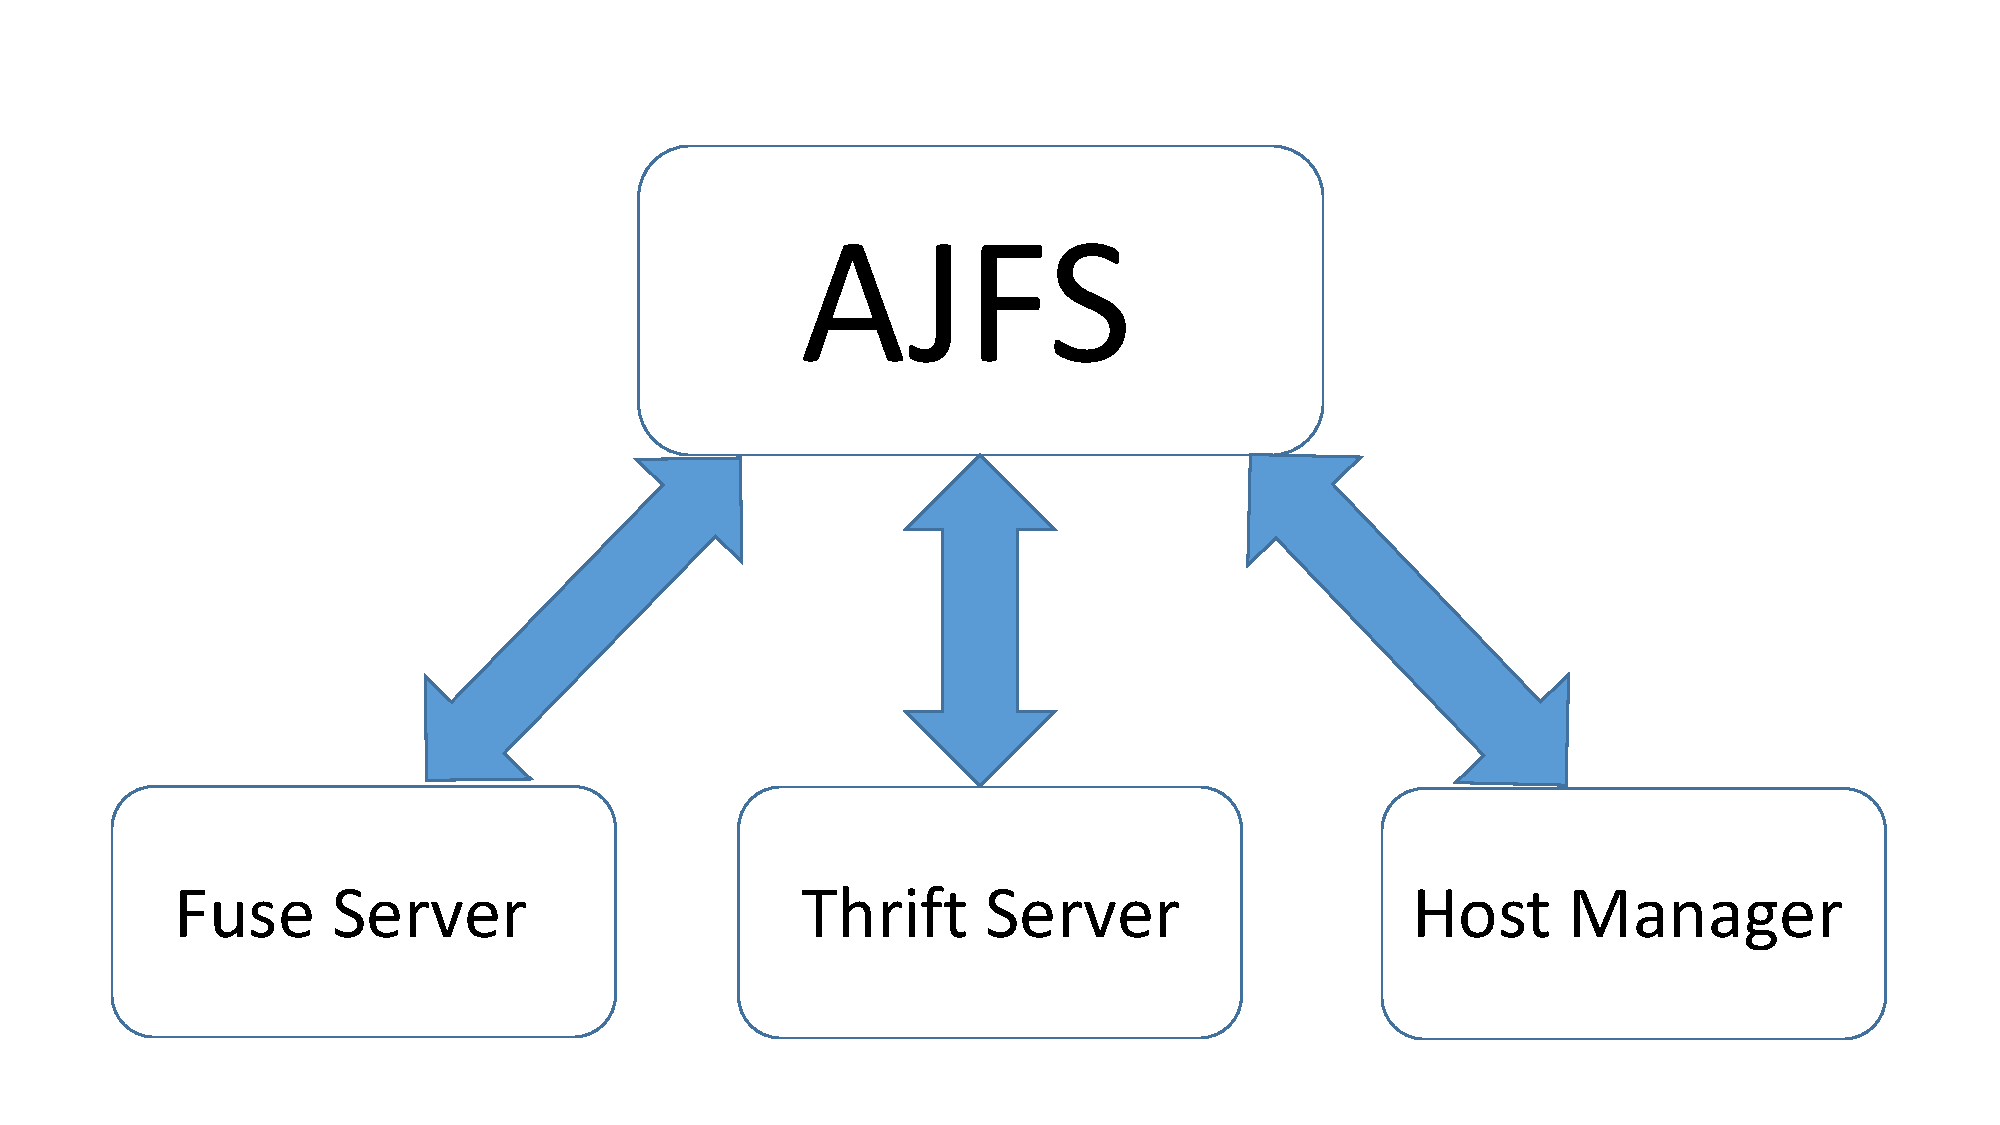
\includegraphics[width=\linewidth]{architecture.pdf}
\caption{AJFS system architecture}
\label{fig:architecture}
\vspace{-5mm}
\end{figure}
